% sections/metodologia.tex
\section{Metodologia}

\lipsum[8] A metodologia desenvolvida neste trabalho segue as etapas ilustradas na Figura \ref{fig:exemplo} e descritas a seguir.

\subsection{Coleta de Dados}

\lipsum[9] Os dados foram coletados através de simulações computacionais utilizando parâmetros específicos. A Tabela \ref{tab:parametros} apresenta os principais parâmetros utilizados nas simulações.

\begin{table}[H]
\centering
\caption{Parâmetros utilizados nas simulações computacionais}
\label{tab:parametros}
\begin{tabular}{@{}lccl@{}}
\toprule
\textbf{Parâmetro} & \textbf{Símbolo} & \textbf{Valor} & \textbf{Unidade} \\ \midrule
Tempo de simulação & $T_{sim}$ & 1000 & s \\
Passo de integração & $\Delta t$ & 0.01 & s \\
Número de iterações & $N_{iter}$ & 10000 & - \\
Tolerância & $\epsilon$ & $10^{-6}$ & - \\
Fator de amortecimento & $\zeta$ & 0.15 & - \\
Frequência natural & $\omega_n$ & 25.0 & rad/s \\
\bottomrule
\end{tabular}
\end{table}

\subsection{Processamento e Análise}

\lipsum[10] O processamento dos dados seguiu um protocolo rigoroso de análise estatística. Os métodos numéricos clássicos foram implementados, incluindo o método de Euler, cuja equação fundamental é expressa como:

\begin{equation}
\frac{dy}{dt} = f(t, y), \quad y(t_0) = y_0
\label{eq:euler}
\end{equation}

onde $f(t, y)$ representa a função que descreve o sistema dinâmico. Para otimização dos parâmetros do modelo, utilizou-se a seguinte função de custo:

\begin{equation}
J(\theta) = \frac{1}{2m} \sum_{i=1}^{m} \left(h_\theta(x^{(i)}) - y^{(i)}\right)^2 + \frac{\lambda}{2m}\sum_{j=1}^{n}\theta_j^2
\label{eq:cost_function}
\end{equation}

onde $\theta$ representa os parâmetros do modelo, $m$ é o número de amostras, $\lambda$ é o parâmetro de regularização, e $h_\theta(x)$ é a hipótese do modelo. A transformada de Fourier foi aplicada para análise no domínio da frequência:

\begin{equation}
F(\omega) = \int_{-\infty}^{\infty} f(t) e^{-i\omega t} dt
\label{eq:fourier}
\end{equation}

\begin{figure}[H]
\centering
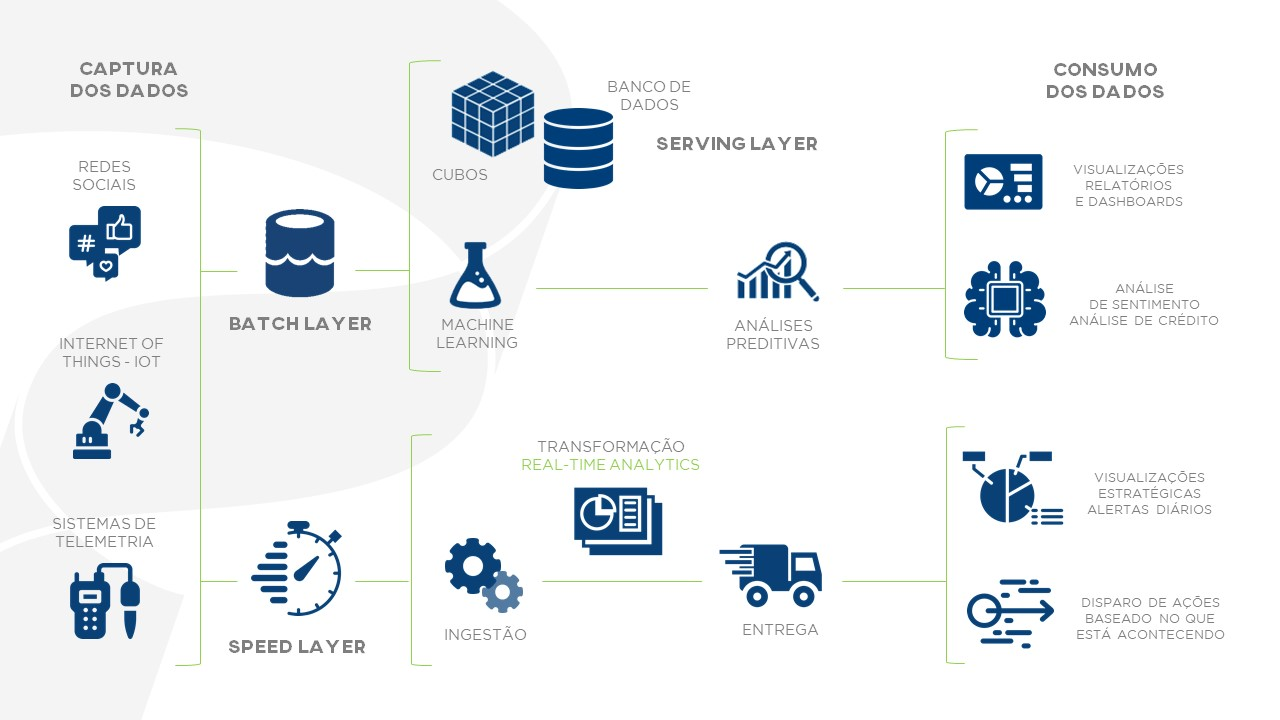
\includegraphics[width=0.7\textwidth]{images/img_001.jpg}
\caption{Exemplo de visualização dos resultados obtidos através da metodologia proposta. A figura ilustra o comportamento do sistema ao longo do tempo.}
\label{fig:exemplo}
\end{figure}
